\documentclass[t,10pt,a3paper]{beamer} %,a4paper %aspectratio=169
\usepackage[utf8]{inputenc}

\usepackage{pslatex}

%\usepackage[left=2cm,right=2cm,top=3cm,bottom=1.5cm]{geometry} % page settings
\usepackage{amsmath} 	% provides many mathematical environments & tools
\usepackage{mathdots} 
\usepackage{amsfonts}
\usepackage{amssymb}
\usepackage{chemist} 	% pour les formules chimiques. 
\usepackage{hyperref}	% pour les hyperliens. 
\usepackage{moreverb}	% pour verbatimtab.
\usepackage{graphicx} 	% pour insérer des images.
%\usepackage{subfigure} 	% pour faire des sous-figures.
\usepackage{caption}    % ---
\usepackage{subcaption} % ---
\usepackage[bb=dsserif]{mathalpha}  % for the 1 characteristics function
\usepackage{bm}                     % for the 1 characteristics function
%\usepackage{fullpage} 	% pour la page de garde. 
%\usepackage{eso-pic} 	% pour la page de garde.
\usepackage{pgf, tikz, tkz-euclide}	% pour les figures/schémas.
	\usetikzlibrary{arrows,shapes,positioning}
	\usetikzlibrary{calc,angles,quotes}
    \usetikzlibrary{patterns}

	
\usepackage{verbatim}
	
%\usepackage{multimedia} % pour les vidéos.
\usepackage{movie15} 	%insertion de vidéos dans le pdf

%\usepackage{biblatex} %Imports biblatex package
%\addbibresource{biblio/biblio.bib} %Import the bibliography file
%\bibliographystyle{amsalpha}

% TEMPLATE ...........................................
%\usetheme{Warsaw}
%\usecolortheme{default}
\usetheme{CambridgeUS}
%\usetheme{AnnArbor}
\usecolortheme{seahorse} %beaver crane 

%\setlength{\parindent}{0mm}%0.5in

% NEW TEMPLATE .......................................
%\usetheme{SimplePlusAIC}
%\usepackage{booktabs} % Allows the use of \toprule, \midrule and  \bottomrule in tables
%\usepackage{svg} %allows using svg figures
%\usepackage{makecell}
%\newcommand*{\defeq}{\stackrel{\text{def}}{=}}

%Select the Epilogue font (requires luaLatex or XeLaTex compilers)
%\usepackage{fontspec}
%\setsansfont{Epilogue}[
%    Path=./epilogueFont/,
%    Scale=0.9,
%    Extension = .ttf,
%    UprightFont=*-Regular,
%    BoldFont=*-Bold,
%    ItalicFont=*-Italic,
%    BoldItalicFont=*-BoldItalic
%    ]
% ..................................................


% PARAMETRES =======================================================================

\setbeamersize{
  text margin left 		= 1cm, % normalement c'est 1 cm
  text margin right 	= 1cm, % normalement c'est 1 cm
  sidebar width left	= 0cm,
  sidebar width right	= 0cm
}


% Nouvelles couleurs :
\definecolor{vert}{rgb}{0.21,0.56,0.55}
\definecolor{rouge}{rgb}{0.74,0.08,0.128}

%\definecolor{ffxfqq}{rgb}{1,0.4980392156862745,0}
%\definecolor{ttttff}{rgb}{0.2,0.2,1}
%\definecolor{qqffqq}{rgb}{0,1,0}
%\definecolor{ffqqqq}{rgb}{1,0,0}
%\definecolor{wrwrwr}{rgb}{0.3803921568627451,0.3803921568627451,0.3803921568627451}
%\definecolor{rvwvcq}{rgb}{0.08235294117647059,0.396078431372549,0.7529411764705882}





% Couleurs du diapo :
%\setbeamercolor{normal text}{fg=black,bg=white}
\setbeamercolor{alerted text}{fg=vert}
%\setbeamercolor{example text}{fg=green!50!black}
\setbeamercolor{structure}{fg=vert!90} % beamer@blendedblue d'où ce bleu par défaut
%\setbeamercolor{background canvas}{parent=normal text}
  
\setbeamertemplate{footline}[frame number]

% Pour des diapos cachées : 
\newcommand{\backupbegin}{
  \newcounter{framenumberappendix}
  \setcounter{framenumberappendix}{\value{framenumber}}
  \setbeamertemplate{footline}{}
}
\newcommand{\backupend}{
  \addtocounter{framenumberappendix}{-\value{framenumber}}
  \addtocounter{framenumber}{\value{framenumberappendix}}
  \setbeamertemplate{footline}{
    \vspace{-1cm}\small{\insertframenumber/\inserttotalframenumber}
  }
}
  
\setbeamertemplate{navigation symbols}{%
\insertslidenavigationsymbol
\insertframenavigationsymbol
\insertsubsectionnavigationsymbol
\insertsectionnavigationsymbol
\insertdocnavigationsymbol
\insertbackfindforwardnavigationsymbol
}

\setbeamerfont{subsection in toc}{size=\footnotesize}

% pour élargir la surface utile dans beamer
\newenvironment{changemargin}[2]{%  
 \begin{list}{}{%
     \setlength{\topsep}{0pt}%
     \setlength{\leftmargin}{#1}%
     \setlength{\rightmargin}{#2}%
     \setlength{\listparindent}{\parindent}%
     \setlength{\itemindent}{\parindent}%
     \setlength{\parsep}{\parskip}%
   }%
\item[]}{\end{list}}

% pour élargir la surface utile dans beamer
\newenvironment{changemargin_top}[3]{%  
 \begin{list}{}{%
     \setlength{\topsep}{0pt}%
     \setlength{\leftmargin}{#1}%
     \setlength{\rightmargin}{#2}%
     \setlength{\topmargin}{#3}%
     \setlength{\listparindent}{\parindent}%
     \setlength{\itemindent}{\parindent}%
     \setlength{\parsep}{\parskip}%
   }%
\item[]}{\end{list}}

% POUR UTILISER LA MACRO: ^
% \begin{changemargin}{-0.5cm}{-0.5cm} % en début de frame (juste après \frametitle{})
% \end{changemargin}      


   
\title{ \textbf{\textsc{ }} \\\rule{\linewidth}{0.1mm} }
\subtitle{ \\ \quad }
\author{Pauline \textsc{Vidal}}
\date{}



% DOCUMENT ===============================================================================

\begin{document}



\frame[plain]{  % --------------------------------------------------------------------------------
	\vspace*{2.5cm}	
	\centering
	\Large Meshing strategy in GYSELA
	%\rule{\linewidth}{0.1mm}
	%\vspace*{0.5cm}
	
	\normalsize
	\begin{center}
		\color{vert!30} \rule{10cm}{0.3mm}
	\end{center}
	
	\normalsize
	\textsc{26 Avril 2024}
	
	\vspace*{0.7cm}
	Alexander \textsc{Hoffmann}, Pauline \textsc{Vidal}
	
	\vspace*{1cm}
	\footnotesize
	%Eric \textsc{Sonnendrücker},
	%Michel \textsc{Mehrenberger},
	%Virginie \textsc{Grandgirard}
	
}

\fontsize{8}{8}



\frame{  % --------------------------------------------------------------------------------
\frametitle{\color{vert} Contents}	
	\footnotesize 
	
	\tableofcontents[firstsection=1, sectionstyle=show,subsectionstyle=shaded, subsubsectionstyle=hide] 
}

\section{Needs for the mesher}
\begin{frame} % --------------------------------------------------------------------------------
\frametitle{\color{vert}\textbf{Needs for the mesher}}
\footnotesize	

\vspace*{0.25cm}
{\color{vert}$\blacktriangleright$ }
\textbf{For Valsov Poisson equations:}

\vspace*{0.15cm}

\qquad {\color{vert}$\triangleright$} Spline representation of the mapping (splines or NURBS coefficients). \par 

\vspace*{0.15cm}
\qquad {\color{vert}$\triangleright$} Connections between patches: \par 
\qquad \qquad {\color{vert}$\bullet$} Interfaces of each patch: list of faces, edges and corners of each patch; \par
\qquad \qquad {\color{vert}$\bullet$}  Connection of these interfaces with the other interfaces. \par 

\vspace*{0.15cm}
\qquad {\color{vert}$\triangleright$} List of special points (coordinates O-points, X-points ...).


\end{frame}


\section{SOLEDGE mesher}
	\begin{frame} % --------------------------------------------------------------------------------
	\frametitle{\color{vert}\textbf{SOLEDGE mesher}}

	%\vspace*{0.25cm}
	Summary of the SOLEDGE3X mesher given by Hugo Bufferand:
	\begin{itemize}
		\item SOLEDGE3X mesher idea is rather basic ("without mathematical strategy")
		\item It searches only for intersections of the coordinate lines 
				$\rightarrow$ No mapping is computed
		\item Fulfills the current demands for SOLEDGE, but not optimized
		\item No documentation about how it is working
		\item Complete rewrite is desired at some point
	\end{itemize}

	\begin{alertblock}{\large{Implication for usage}}
		Since only the mesh is computed, this can not be used for an
		isogeometric analysis type approach.
	\end{alertblock}


\end{frame}

\section{SOLEDGE mesher}
	\begin{frame} % --------------------------------------------------------------------------------
	\frametitle{\color{vert}\textbf{SOLEDGE mesher}}
	\footnotesize	

	%\vspace*{0.25cm}
	{\color{vert}$\blacktriangleright$ }
	\textbf{In \verb|Mailleur\_SOLEDGE| folder:} \par
	\qquad {\color{vert} $\rightarrow$} Tutorial videos and Matlab code. \par 
	\qquad {\color{vert} $\rightarrow$} Example of mesh: \verb|routines/mesh.h5| \par 

	\vspace*{0.15cm}

	{\color{vert}$\triangleright$ }
	In \verb|routines/mesh.h5|: \par 
	\begin{columns}
	\scriptsize
	\begin{column}{0.3\textwidth}
	\begin{itemize}
		\item[\verb|NMegazones|] [int] number of megazone.
		\item[\verb|NZones|] [int] number of patch. 
		\item[\verb|config|] [Group] configuration parameters used to build the mesh.
		\item[6 \verb|megazone1|] [Group] information about each megazone. 
		\item[\verb|wall|] [Group] physical coordinates $(R,Z)$ of the wall. 
		\item[28 \verb|zone1|] [Group] information about each patch. 
	\end{itemize}

	\vspace*{0.15cm}
	{\color{vert} $\bullet$}  In \verb|wall|: \par 
	\ \verb|R| and \verb|Z| [array 33]; \par 

	\end{column}
	\begin{column}{0.6\textwidth}
	{\color{vert} $\bullet$} In \verb|config|: \par 
	\ \verb|nsep| [int]; \par 
	\ \verb|psi| [array (501x601)]; \par 
	\ \verb|psicore|, \verb|psiep1| and \verb|psiep2| [float]; \par 
	\ \verb|r| and \verb|z|  [array 501x601]; \par 


	\vspace*{0.15cm}
	{\color{vert} $\bullet$}  In \verb|megazone1|: \textit{[not used anymore]} \par 
	\ \verb|configuration| [array 5]; \par 
	\ \verb|isperiodic| [int]; \par 
	\ \verb|size| [int]; \par 

	\vspace*{0.15cm}

	{\color{vert} $\bullet$}  In \verb|zones1|: \par
	\ \verb|Bphi|, \verb|Br| and \verb|Bz| [array 41x21]: magnetic field at the center of cells; \par 
	\ \verb|MagNeighbors| and \verb|Neighbors| [Group of 4 [int]]: neighbors of the patch in ENSW directions; \par 
	\ \verb|Nx| and \verb|Ny| [int]; \par 
	\ \verb|Rcorner| and \verb|Zcorner| [array 40x20]: physical mesh points; \par 
	\ \verb|Rgeom| and \verb|Zgeom| [array 41x21]; \par 
	\ \verb|chi| [array 39x19]: mask function defines in wall or in plasma; \par 
	\ \verb|x|, \verb|z|, \verb|xm|, \verb|zm|, \verb|xp|, \verb|zp| [array 39x19]: logical mesh points; \par 
	\ \verb|xmax|, \verb|xmin|, \verb|zmax|, \verb|zmin| [float]. \par
	\end{column}
	\end{columns}


\end{frame}



\begin{frame} % --------------------------------------------------------------------------------
\frametitle{\color{vert}\textbf{SOLEDGE mesher}}
\footnotesize	

%\vspace*{0.25cm}
{\color{vert}$\blacktriangleright$ }
\textbf{Display data:} (\verb|x|, \verb|z|) and (\verb|Rcorner|, \verb|Zcorner|)

\vspace*{0.25cm}
\begin{changemargin}{-2cm}{-2cm} 
\begin{center}
\begin{figure}[!h]
	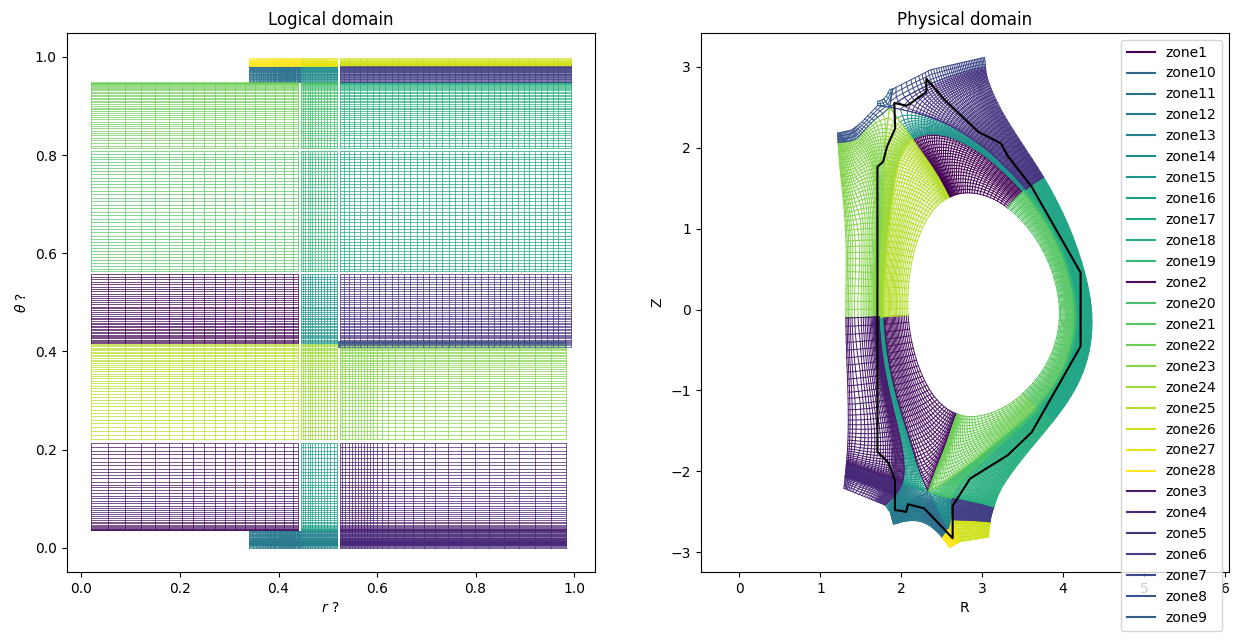
\includegraphics[width=1.15\textwidth]{images/mesher_logical_physical_mesh.png}
\end{figure}	
\end{center}
\end{changemargin}

\end{frame}


\begin{frame} % --------------------------------------------------------------------------------
\frametitle{\color{vert}\textbf{SOLEDGE mesher}}
\footnotesize	

%\vspace*{0.25cm}
{\color{vert}$\blacktriangleright$ }
\textbf{Display data:} Differences between (\verb|x|, \verb|z|), (\verb|xm|, \verb|zm|) and (\verb|xp|, \verb|zp|)
\begin{changemargin}{-2cm}{-2cm} 
\begin{center}
\begin{figure}[!h]
	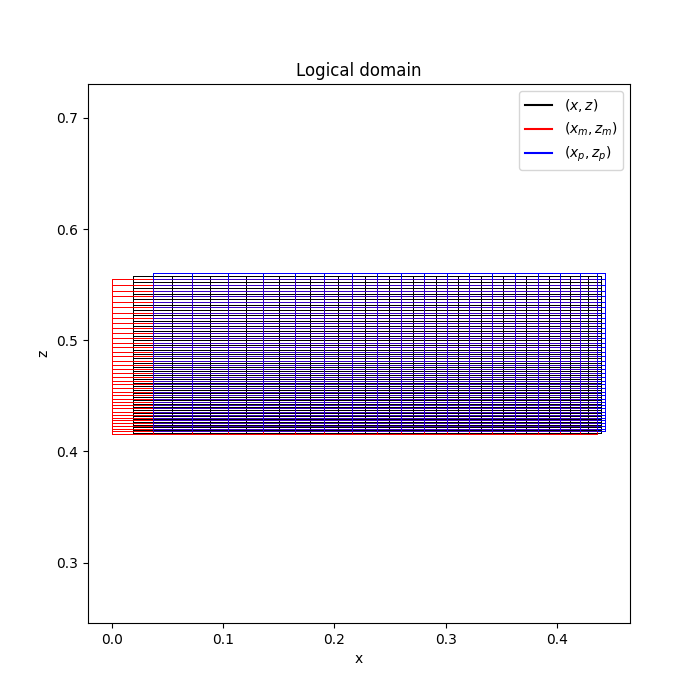
\includegraphics[width=0.7\textwidth]{images/Diff_zwischen_x_xm_xp.png}
\end{figure}	
\end{center}
\end{changemargin}

\end{frame}

\begin{frame} % --------------------------------------------------------------------------------
\frametitle{\color{vert}\textbf{SOLEDGE mesher}}
\footnotesize	

%\vspace*{0.25cm}
{\color{vert}$\blacktriangleright$ }
\textbf{Display data:} (\verb|Rgeom|, \verb|Zgeom|)
\begin{changemargin}{-2cm}{-2cm} 
\begin{center}
\begin{figure}[!h]
	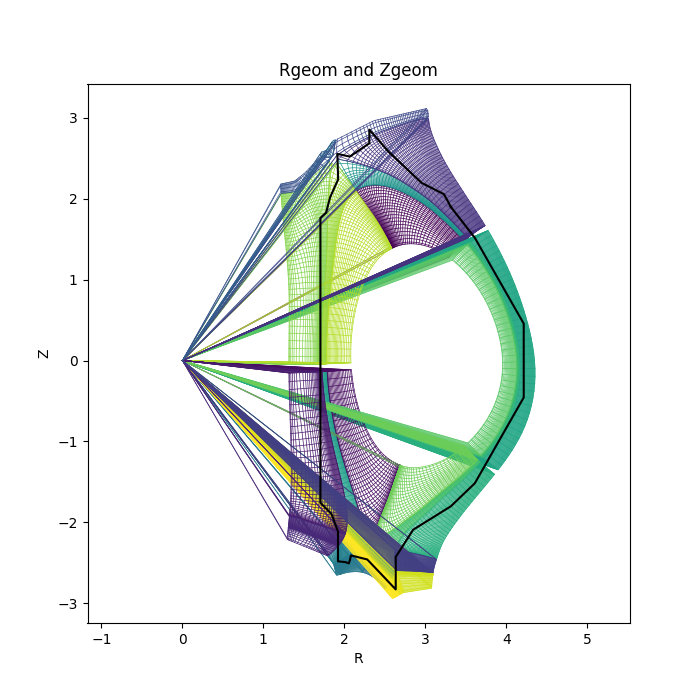
\includegraphics[width=0.7\textwidth]{images/Rgeom_and_Zgeom.png}
\end{figure}	
\end{center}
\end{changemargin}

\end{frame}



\begin{frame} % --------------------------------------------------------------------------------
\frametitle{\color{vert}\textbf{SOLEDGE mesher}}
\footnotesize	

%\vspace*{0.25cm}
{\color{vert}$\blacktriangleright$ }
\textbf{Display data:} Example of X-point
\begin{changemargin}{-2cm}{-2cm} 
\begin{center}
\begin{figure}[!h]
	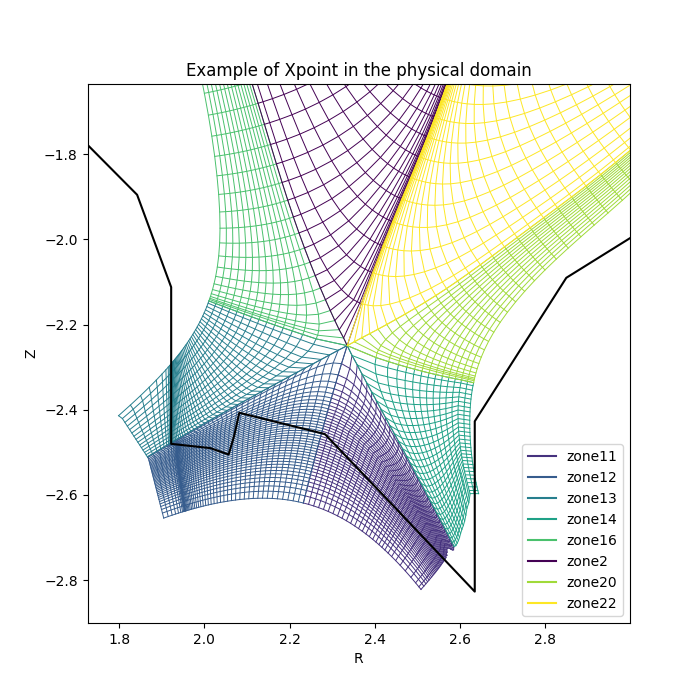
\includegraphics[width=0.7\textwidth]{images/Example_of_Xpoint.png}
\end{figure}	
\end{center}
\end{changemargin}

\end{frame}


\section{TOKAMESH}

\begin{frame} % --------------------------------------------------------------------------------
\frametitle{\color{vert}\textbf{TOKAMESH}}
\footnotesize	

\vspace*{0.25cm}
Report which mostly explains the underlying theory and algorithm: 
\textit{Tokamesh : A software for mesh generation in Tokamaks}, 
Hervé Guillard, Jalal Lakhlili, Adrien Loseille, Alexis Loyer, Boniface Nkonga, Ahmed Ratnani and Ali Elarif. December 2018. 
\vspace*{0.5 cm}

{\color{vert}$\blacktriangleright$ }
\textbf{Mathematical idea}
\begin{itemize}
	\item Uses advanced mathematical ideas from Morse theory to compute the patches
	\item Spline mappings are computed for each patch
	\item Mappings are $C^1$-conforming away from the X-point
\end{itemize}

{\color{vert}$\blacktriangleright$ }
\textbf{Code}

\begin{itemize}
	\item INRIA repository is not accessible $\rightarrow$ did not get access to the code not so far
\end{itemize}

\end{frame}



\end{document}